\documentclass[11pt,a4paper]{article}

% Image mode: pdf.
% Image paths stay relative. In PDF mode, place same-basename PDF conversions
% of the chapter SVG files in the assets/ directory beside this source.

\usepackage{iftex}
\ifPDFTeX
  \PackageError{handout}{This template requires XeTeX or Tectonic}{Compile with xelatex or tectonic.}
\fi

\usepackage[a4paper,top=18mm,bottom=20mm,left=20mm,right=20mm,headsep=6mm]{geometry}
\usepackage{fontspec}
\usepackage{xeCJK}
\usepackage{amsmath}
\usepackage{unicode-math}

% Font settings are intentionally visible in the generated .tex file.
% These defaults target the macOS machine used for the released PDF.
% Change the family names when compiling on another system.
\setmainfont{Songti TC}
\setsansfont{Heiti TC}
\setmonofont{Menlo}
\setCJKmainfont{Songti TC}
\setCJKsansfont{Heiti TC}
\setCJKmonofont{Heiti TC}
\setmathfont{STIX Two Math}
\XeTeXlinebreaklocale "zh"
\XeTeXlinebreakskip=0pt plus 1pt

\usepackage{xcolor}
\definecolor{HandoutBlue}{HTML}{215A91}
\definecolor{HandoutBlueLight}{HTML}{EEF5FC}
\definecolor{HandoutGreen}{HTML}{39715A}
\definecolor{HandoutGreenLight}{HTML}{EFF8F3}
\definecolor{HandoutGold}{HTML}{8A641C}
\definecolor{HandoutGoldLight}{HTML}{FFF8E8}
\definecolor{HandoutInk}{HTML}{253142}
\definecolor{HandoutMuted}{HTML}{667085}

\usepackage{graphicx}
\makeatletter
% Pandoc 3 emits an accessibility `alt` key for raster/PDF images. Older
% graphicx releases do not know that key, so accept it without changing layout.
\@ifundefined{KV@Gin@alt}{\define@key{Gin}{alt}{}}{}
\newsavebox\pandoc@box
\newcommand*\pandocbounded[1]{%
  \sbox\pandoc@box{#1}%
  \Gscale@div\@tempa{\textheight}{\dimexpr\ht\pandoc@box+\dp\pandoc@box\relax}%
  \Gscale@div\@tempb{\linewidth}{\wd\pandoc@box}%
  \ifdim\@tempb\p@<\@tempa\p@\let\@tempa\@tempb\fi
  \ifdim\@tempa\p@<\p@\scalebox{\@tempa}{\usebox\pandoc@box}%
  \else\usebox{\pandoc@box}%
  \fi
}
\makeatother
\usepackage{float}
\floatplacement{figure}{H}
% Pandoc uses LTcaptype=none for uncaptioned longtables. The caption package
% expects that name to exist as a counter even though it is never displayed.
\newcounter{none}
\usepackage{caption}
\captionsetup[figure]{labelformat=empty,labelsep=none,font=small}

\usepackage{booktabs,longtable,array,calc}
\usepackage{etoolbox}
\makeatletter
\patchcmd\longtable{\par}{\if@noskipsec\mbox{}\fi\par}{}{}
\makeatother

\usepackage[most]{tcolorbox}
\tcbuselibrary{breakable,skins}
\newtcolorbox{HandoutLearningMap}{
  enhanced,breakable,colback=HandoutBlueLight,colframe=HandoutBlue,
  boxrule=0.8pt,arc=1.5mm,left=3mm,right=3mm,top=2mm,bottom=2mm,
  before skip=8pt,after skip=10pt
}
\newtcolorbox{HandoutWorkedExample}{
  enhanced,breakable,colback=HandoutGreenLight,colframe=HandoutGreen,
  boxrule=0.65pt,arc=1.5mm,left=3mm,right=3mm,top=2mm,bottom=2mm,
  before skip=8pt,after skip=10pt
}
\newtcolorbox{HandoutSelfCheck}{
  enhanced,breakable,colback=HandoutGoldLight,colframe=HandoutGold,
  boxrule=0.65pt,arc=1.5mm,left=3mm,right=3mm,top=2mm,bottom=2mm,
  before skip=8pt,after skip=10pt
}

\usepackage{titlesec}
\titleformat{\section}{\sffamily\bfseries\Large\color{HandoutBlue}}{}{0pt}{}
\titleformat{\subsection}{\sffamily\bfseries\large\color{HandoutInk}}{}{0pt}{}
\titleformat{\subsubsection}{\sffamily\bfseries\normalsize\color{HandoutInk}}{}{0pt}{}
\titlespacing*{\section}{0pt}{1.4em}{0.55em}
\titlespacing*{\subsection}{0pt}{1.15em}{0.45em}
\titlespacing*{\subsubsection}{0pt}{0.9em}{0.35em}
\setcounter{secnumdepth}{-\maxdimen}

\usepackage{hyperref}
\usepackage{bookmark}
\IfFileExists{xurl.sty}{\usepackage{xurl}}{}
\urlstyle{same}
\hypersetup{
  colorlinks=true,
  linkcolor=HandoutBlue,
  urlcolor=HandoutBlue,
  citecolor=HandoutBlue,
  pdftitle={數1-3 多項式函數},
  pdfsubject={數學},
  pdfcreator={Pandoc with the HighSchooContent LaTeX template}
}

\setlength{\parindent}{0pt}
\setlength{\parskip}{0.55em plus 0.15em minus 0.1em}
\setlength{\emergencystretch}{3em}
\setlength{\LTpre}{0.5em}
\setlength{\LTpost}{0.5em}
\renewcommand{\arraystretch}{1.18}
\providecommand{\tightlist}{%
  \setlength{\itemsep}{0pt}\setlength{\parskip}{0pt}}
\pagestyle{plain}


\begin{document}

\begin{tcolorbox}[
  enhanced,colback=white,colframe=HandoutBlue,boxrule=1.1pt,arc=2mm,
  borderline west={3pt}{0pt}{HandoutBlue},left=5mm,right=4mm,top=4mm,bottom=4mm
]
{\sffamily\small\bfseries\color{HandoutBlue}學生講義}\par
{\sffamily\bfseries\LARGE\color{HandoutInk}數1-3 多項式函數}\par
\vspace{0.35em}{\large 用除法、圖形與符號分析連結多項式的局部資訊和整體行為}\par
\vspace{0.45em}{\small\color{HandoutMuted}%
科目：數學
\quad 課程：普通高中數學 第一冊
\quad 版本：學生版｜核心＋理解
\quad 校訂：2026-08-29
}\par
\vspace{0.25em}{\small\color{HandoutMuted}範圍：114 學年度數學第一冊第 3 章；多項式運算、簡單多項式函數、三次圖形與多項式不等式}\par
\end{tcolorbox}


\begin{HandoutLearningMap}

\subsection{本章問題與能力}\label{ux672cux7ae0ux554fux984cux8207ux80fdux529b}

\begin{enumerate}
\def\labelenumi{\arabic{enumi}.}
\tightlist
\item
  多項式的係數、次數與四則運算如何形成一套穩定的代數語言？
\item
  除法原理、綜合除法、餘式定理與因式定理如何互相連結？
\item
  坐標對稱、函數記號與平移如何把方程式轉成可讀的圖形？
\item
  配方、判別式與閉區間如何決定二次函數的頂點、交點與極值？
\item
  三次函數的標準形、對稱中心、大域特徵與局部一次近似如何取得？
\item
  多項式的根與重數如何控制不等式的正負區間？
\end{enumerate}

本章路徑：多項式語言 → 除法與餘式 → 函數與圖形 → 二次函數 → 三次函數 → 多項式不等式。

\end{HandoutLearningMap}

\section{0. 本章實際用途：校正、最佳化與可行範圍}\label{ux672cux7ae0ux5be6ux969bux7528ux9014ux6821ux6b63ux6700ux4f73ux5316ux8207ux53efux884cux7bc4ux570d}

多項式可用來描述輸入與輸出之間的關係。感測器在一小段操作範圍內，常用一次或二次多項式校正讀值；產品的收益、面積或能耗模型常形成二次式，頂點便對應最佳配置；已知若干測試值時，餘式定理可直接抽取指定輸入的資訊。

圖形提供整體判讀。二次函數的開口、頂點與交點可說明一項設計在何處達到最大或最小；三次函數的最高次項決定遠端趨勢，平移後的標準形則顯示對稱中心。當系統只在某個基準值附近運作時，連續綜合除法可把多項式寫成基準位移的次方，保留常數項與一次項便得到容易計算的局部近似。

不等式回答「哪些輸入符合條件」。成本低於上限、面積高於門檻、訊號維持正值，都可整理成多項式的正負問題。根把數線分段，根的重數決定經過該點時是否變號。

\section{1. 多項式的語言與運算}\label{ux591aux9805ux5f0fux7684ux8a9eux8a00ux8207ux904bux7b97}

\subsection{1.1 定義、係數與次數}\label{ux5b9aux7fa9ux4fc2ux6578ux8207ux6b21ux6578}

一元多項式可寫成

\[
f(x)=a_nx^n+a_{n-1}x^{n-1}+\cdots+a_1x+a_0,
\]

其中 \(n\) 是非負整數，各係數 \(a_i\) 是實數。當 \(a_n\ne0\) 時，\(n\) 稱為 \(f\) 的\textbf{次數}，記作 \(\deg f=n\)；\(a_n\) 是首項係數，\(a_0\) 是常數項。非零常數是零次多項式；零多項式的次數不定義。

多項式中的指數皆為非負整數。因此 \(3x^4-\sqrt2x+1\) 是四次多項式，而含有 \(x^{-1}\)、\(\sqrt{x}\) 或變數位於分母的式子不屬於多項式。

兩個多項式相等的條件，是每一個相同次方的係數都相等。缺少的次方項以係數 \(0\) 表示，這個表示法在比較係數與綜合除法中都很重要。

\subsection{1.2 加、減、乘與代值}\label{ux52a0ux6e1bux4e58ux8207ux4ee3ux503c}

加減法將同次項係數相加減；乘法由分配律展開後合併同次項。若 \(f,g\) 都是非零多項式，則

\[
\deg(fg)=\deg f+\deg g.
\]

理由是兩者最高次項 \(a_nx^n\)、\(b_mx^m\) 相乘得到 \(a_nb_mx^{n+m}\)，且 \(a_nb_m\ne0\)。加減時最高次項可能互相消去，所以

\[
\deg(f\pm g)\le \max\{\deg f,\deg g\}.
\]

把 \(x=t\) 代入 \(f(x)\) 所得的數記作 \(f(t)\)。代值可以表示資料模型在指定輸入的輸出，也會在餘式定理中直接出現。

\subsection{例 1｜由相等多項式決定係數}\label{ux4f8b-1ux7531ux76f8ux7b49ux591aux9805ux5f0fux6c7aux5b9aux4fc2ux6578}

已知

\[
(a+1)x^3+(b-2)x^2+3x+2=3x+2,
\]

求 \(a,b\)。

右式的三次項與二次項係數都是 \(0\)。逐項比較得

\[
a+1=0,\qquad b-2=0.
\]

所以 \(\boxed{a=-1,\ b=2}\)。

\subsection{例 2｜乘法展開與次數檢查}\label{ux4f8b-2ux4e58ux6cd5ux5c55ux958bux8207ux6b21ux6578ux6aa2ux67e5}

計算 \((2x^2-x+3)(x-2)\)。

\[
\begin{aligned}
(2x^2-x+3)(x-2)
&=2x^3-4x^2-x^2+2x+3x-6\\
&=\boxed{2x^3-5x^2+5x-6}.
\end{aligned}
\]

兩個因式的次數分別為 \(2,1\)，乘積為三次，與結果一致。

\subsubsection{練習 1A}\label{ux7df4ux7fd2-1a}

\begin{enumerate}
\def\labelenumi{\arabic{enumi}.}
\tightlist
\item
  說明 \(3x^4-\sqrt2x+1\) 的次數、首項係數與常數項，並判斷 \(x^{-1}+2\)、\(\sqrt{x}+1\) 是否為多項式。
\item
  若 \((a-1)x^3+(b+2)x^2+4=4\)，求 \(a,b\)。
\item
  展開 \((2x^2-x+3)(x-2)\)。
\item
  設 \(f(x)=x^3-2x+1\)、\(g(x)=-x^3+x^2+4\)，求 \(f(x)+g(x)\) 及其次數。
\item
  一個校正模型為 \(C(t)=2t^3-5t+12\)，求 \(C(3)\)。
\end{enumerate}

\section{2. 除法原理、綜合除法與因式}\label{ux9664ux6cd5ux539fux7406ux7d9cux5408ux9664ux6cd5ux8207ux56e0ux5f0f}

\subsection{2.1 多項式除法原理}\label{ux591aux9805ux5f0fux9664ux6cd5ux539fux7406}

若 \(g(x)\) 是非零多項式，則存在唯一的多項式 \(q(x),r(x)\)，使

\[
\boxed{f(x)=g(x)q(x)+r(x)},
\]

其中 \(r(x)=0\)，或 \(\deg r<\deg g\)。\(q\) 是商，\(r\) 是餘式。

長除法每一步都用目前被除式的最高次項除以除式的最高次項，得到商的一項，再乘回並相減。相減會使最高次降低；有限次後便得到次數低於除式的餘式。

唯一性可由反證確認。若同時有

\[
f=gq_1+r_1=gq_2+r_2,
\]

則 \(g(q_1-q_2)=r_2-r_1\)。若 \(q_1-q_2\) 非零，左側次數至少為 \(\deg g\)；右側次數低於 \(\deg g\)，產生矛盾。因此 \(q_1=q_2\)，進而 \(r_1=r_2\)。

\subsection{例 3｜多項式長除法}\label{ux4f8b-3ux591aux9805ux5f0fux9577ux9664ux6cd5}

求 \(2x^3-3x^2+5\) 除以 \(x^2-x+1\) 的商與餘式。

先補出 \(0x\)。最高次相除得 \(2x\)：

\[
(2x^3-3x^2+0x+5)-2x(x^2-x+1)=-x^2-2x+5.
\]

再以 \(-1\) 乘除式：

\[
(-x^2-2x+5)-(-x^2+x-1)=-3x+6.
\]

因此

\[
\boxed{q(x)=2x-1,\qquad r(x)=-3x+6}.
\]

驗算：\((x^2-x+1)(2x-1)+(-3x+6)=2x^3-3x^2+5\)。

\subsection{\texorpdfstring{2.2 除以 \(x-a\) 與綜合除法}{2.2 除以 x-a 與綜合除法}}\label{ux9664ux4ee5-x-a-ux8207ux7d9cux5408ux9664ux6cd5}

當除式為 \(x-a\) 時，餘式的次數低於 \(1\)，所以餘式是一個常數。綜合除法只記係數，依序執行「首項落下、乘 \(a\)、與下一係數相加」。最後一格是餘式，其餘各格是商的係數。

\begin{figure}
\centering
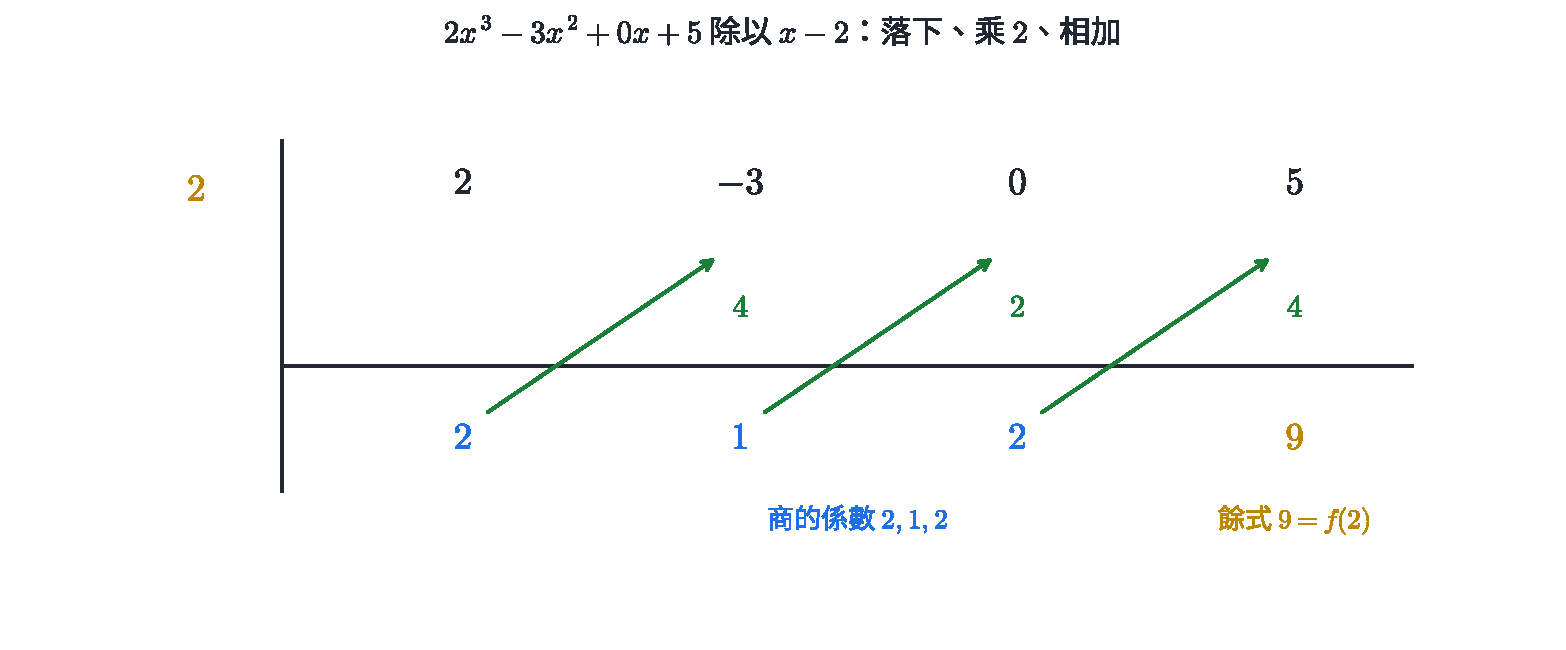
\includegraphics[width=0.92\linewidth,height=\textheight,keepaspectratio,alt={圖 1｜缺少的 x 項補係數 0；最後一格同時是綜合除法餘式與 f(2)。}]{assets/數1-3-綜合除法.pdf}
\caption{圖 1｜缺少的 \(x\) 項補係數 \(0\)；最後一格同時是綜合除法餘式與 \(f(2)\)。}
\end{figure}

\subsection{例 4｜綜合除法與驗算}\label{ux4f8b-4ux7d9cux5408ux9664ux6cd5ux8207ux9a57ux7b97}

用綜合除法計算 \(f(x)=2x^3-3x^2+5\) 除以 \(x-2\)。

係數依序為 \(2,-3,0,5\)，綜合除法底列為 \(2,1,2,9\)，所以

\[
\boxed{q(x)=2x^2+x+2,\qquad r=9}.
\]

展開 \((x-2)(2x^2+x+2)+9\) 可還原 \(f(x)\)。

\subsection{2.3 餘式定理與因式定理}\label{ux9918ux5f0fux5b9aux7406ux8207ux56e0ux5f0fux5b9aux7406}

由除法原理

\[
f(x)=(x-a)q(x)+r
\]

代入 \(x=a\)，得到 \(f(a)=r\)。因此

\[
\boxed{f(x)\text{ 除以 }x-a\text{ 的餘式為 }f(a)}.
\]

這就是\textbf{餘式定理}。若除式為 \(Ax-B\)，其零點為 \(B/A\)，餘式便是

\[
\boxed{f\!\left(\frac BA\right)}.
\]

當餘式為 \(0\) 時得到\textbf{因式定理}：

\[
\boxed{x-a\text{ 是 }f(x)\text{ 的因式}\iff f(a)=0}.
\]

若除式為 \((x-a)(x-b)\) 且 \(a\ne b\)，餘式最高一次，可設為 \(r(x)=mx+n\)。利用 \(r(a)=f(a)\)、\(r(b)=f(b)\) 可解出 \(m,n\)，省去完整長除法。

\subsection{例 5｜由兩個函數值求二次除式的餘式}\label{ux4f8b-5ux7531ux5169ux500bux51fdux6578ux503cux6c42ux4e8cux6b21ux9664ux5f0fux7684ux9918ux5f0f}

已知 \(f(1)=4\)、\(f(-2)=-5\)。求 \(f(x)\) 除以 \((x-1)(x+2)\) 的餘式。

設餘式為 \(r(x)=mx+n\)。在 \(x=1,-2\) 時，除式都為 \(0\)，所以

\[
m+n=4,\qquad -2m+n=-5.
\]

相減得 \(3m=9\)，故 \(m=3,n=1\)。餘式為 \(\boxed{3x+1}\)。

\subsection{例 6｜因式定理重建三次式}\label{ux4f8b-6ux56e0ux5f0fux5b9aux7406ux91cdux5efaux4e09ux6b21ux5f0f}

一首項係數為 \(1\) 的三次多項式 \(f\) 滿足 \(f(1)=f(-2)=0\)、\(f(0)=6\)，且第三個根為 \(r\)。求 \(f(x)\)。

因式定理給出 \(f(x)=(x-1)(x+2)(x-r)\)。代入 \(x=0\)：

\[
(-1)(2)(-r)=2r=6,
\]

所以 \(r=3\)，且 \(\boxed{f(x)=(x-1)(x+2)(x-3)}\)。

\subsection{綜合除法的必要條件}\label{ux7d9cux5408ux9664ux6cd5ux7684ux5fc5ux8981ux689dux4ef6}

標準綜合除法直接適用於除式 \(x-a\)。多項式的每一個次方都要按順序列出係數，缺項以 \(0\) 補齊。這兩項會直接改變商與餘式。

\subsubsection{練習 2A}\label{ux7df4ux7fd2-2a}

\begin{enumerate}
\def\labelenumi{\arabic{enumi}.}
\tightlist
\item
  求 \((x^4-1)\div(x^2+1)\) 的商與餘式。
\item
  用綜合除法求 \((3x^4-2x^2+7)\div(x+1)\)。
\item
  求 \(2x^5-3x+4\) 除以 \(2x-1\) 的餘式。
\item
  若 \(x-2\) 是 \(x^3+ax^2-5x+6\) 的因式，求 \(a\)。
\item
  已知 \(f(x)\) 除以 \(x-1\)、\(x+2\) 的餘式分別為 \(2,-4\)，求 \(f(x)\) 除以 \((x-1)(x+2)\) 的餘式。
\item
  若 \(x^4+ax^3+bx^2+ax+1\) 可被 \(x^2-1\) 整除，求 \(a,b\)。
\end{enumerate}

\section{3. 坐標對稱、函數與基本圖形}\label{ux5750ux6a19ux5c0dux7a31ux51fdux6578ux8207ux57faux672cux5716ux5f62}

\subsection{3.1 坐標對稱與中點}\label{ux5750ux6a19ux5c0dux7a31ux8207ux4e2dux9ede}

點 \(P(a,b)\) 經基本對稱後的坐標為

{\def\LTcaptype{none} % do not increment counter
\begin{longtable}[]{@{}lll@{}}
\toprule\noalign{}
對稱對象 & 像點坐標 & 保留的量 \\
\midrule\noalign{}
\endhead
\bottomrule\noalign{}
\endlastfoot
\(x\) 軸 & \((a,-b)\) & \(x\) 坐標 \\
\(y\) 軸 & \((-a,b)\) & \(y\) 坐標 \\
原點 & \((-a,-b)\) & 到原點距離 \\
直線 \(y=x\) & \((b,a)\) & 交換兩坐標 \\
\end{longtable}
}

若圖形中每一點對稱後仍落在圖形上，該直線稱為對稱軸；若每一點繞某點旋轉 \(180^\circ\) 後仍落在圖形上，該點稱為對稱中心。

兩點 \(A(x_1,y_1)\)、\(B(x_2,y_2)\) 的中點為

\[
\boxed{M\left(\frac{x_1+x_2}{2},\frac{y_1+y_2}{2}\right)}.
\]

每個坐標分別取數線上的平均，便得到線段的中點。

\begin{figure}
\centering
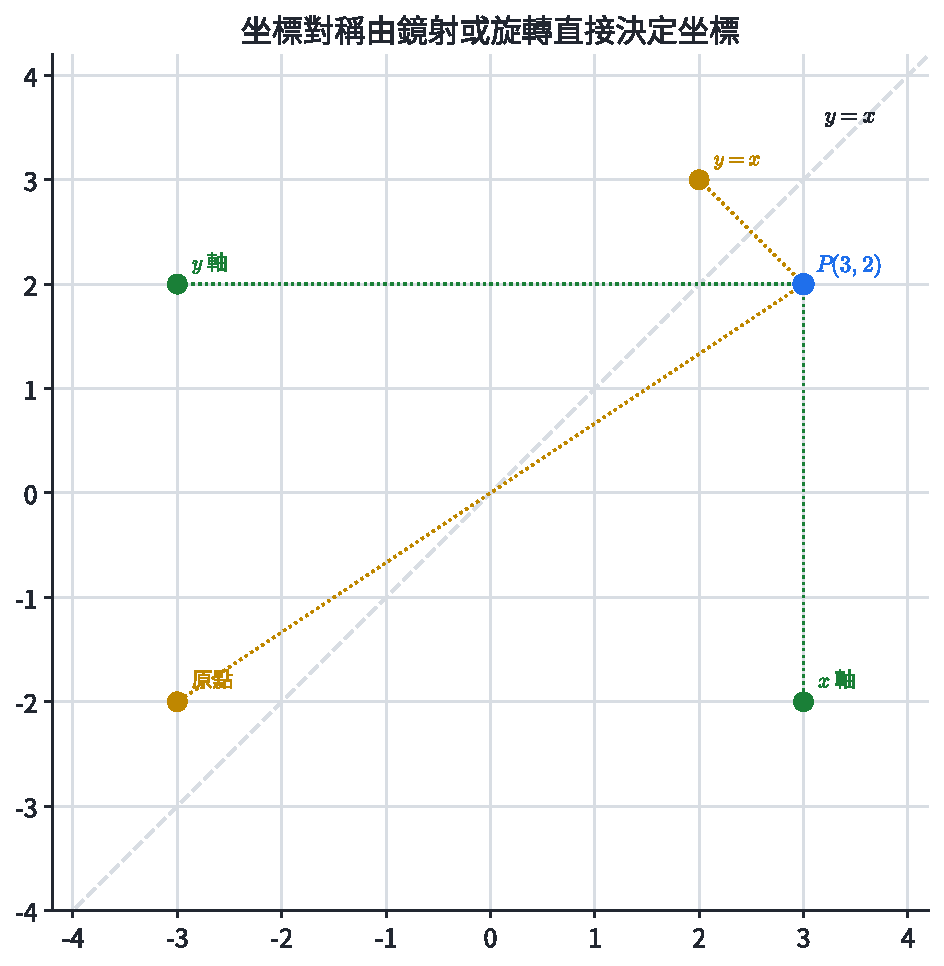
\includegraphics[width=0.76\linewidth,height=\textheight,keepaspectratio,alt={圖 2｜同一點關於坐標軸、原點與 y=x 的像點；虛線連線對應鏡射或旋轉。}]{assets/數1-3-坐標對稱.pdf}
\caption{圖 2｜同一點關於坐標軸、原點與 \(y=x\) 的像點；虛線連線對應鏡射或旋轉。}
\end{figure}

\subsection{3.2 函數、常數函數與一次函數}\label{ux51fdux6578ux5e38ux6578ux51fdux6578ux8207ux4e00ux6b21ux51fdux6578}

若每一個允許的輸入 \(x\) 都恰好對應一個輸出 \(y\)，便稱 \(y\) 是 \(x\) 的函數，記作 \(y=f(x)\)。函數圖形是所有滿足 \(y=f(x)\) 的點 \((x,y)\) 所成的集合。

常數函數 \(f(x)=c\) 的圖形是水平直線 \(y=c\)。一次函數

\[
f(x)=mx+b\qquad(m\ne0)
\]

的圖形是直線，斜率

\[
m=\frac{\Delta y}{\Delta x}
\]

表示輸入每增加一單位，輸出改變多少；\(b=f(0)\) 是 \(y\) 截距。由兩點 \((x_1,y_1)\)、\((x_2,y_2)\) 且 \(x_1\ne x_2\) 可求

\[
m=\frac{y_2-y_1}{x_2-x_1},\qquad b=y_1-mx_1.
\]

\begin{figure}
\centering
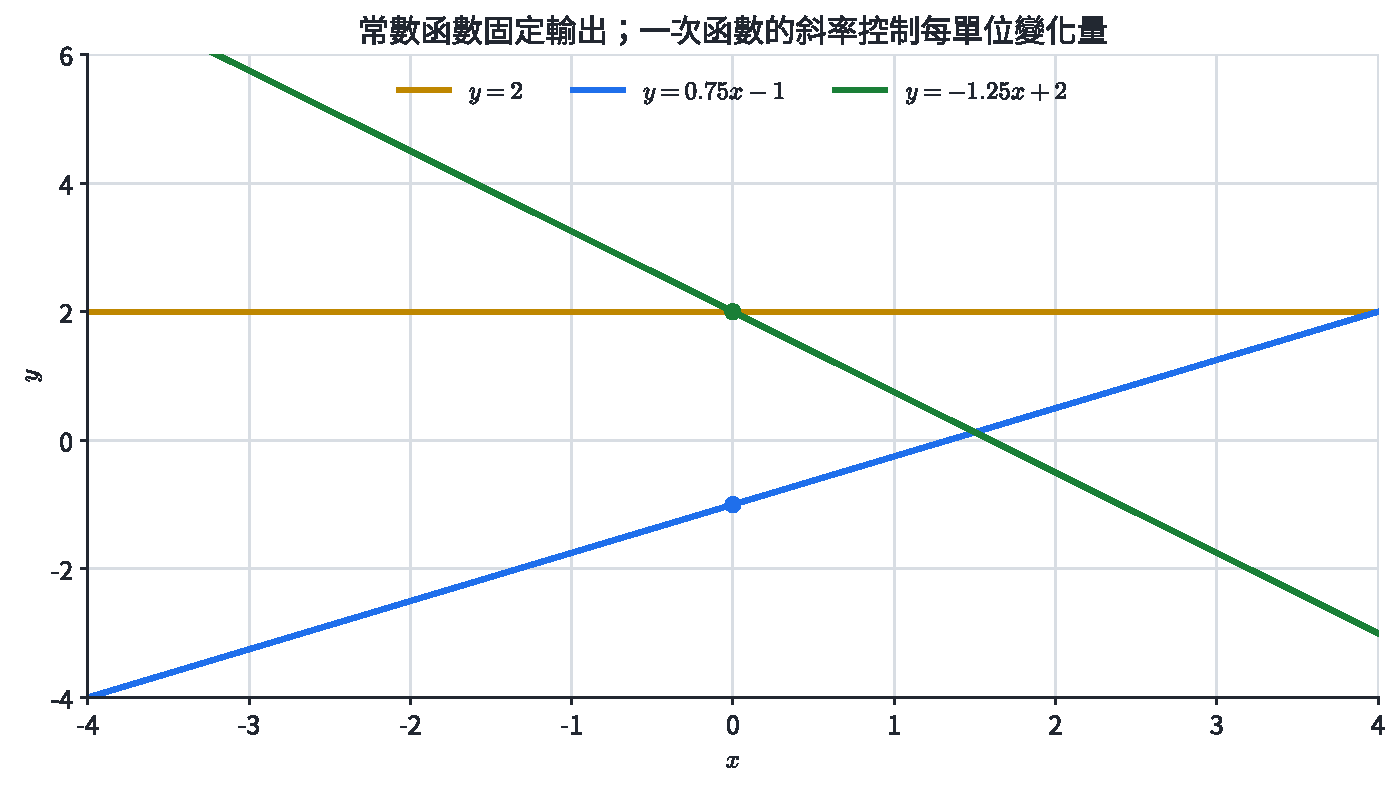
\includegraphics[width=0.88\linewidth,height=\textheight,keepaspectratio,alt={圖 3｜常數函數的輸出固定；兩條一次函數的正負斜率對應遞增與遞減。}]{assets/數1-3-常數與一次函數.pdf}
\caption{圖 3｜常數函數的輸出固定；兩條一次函數的正負斜率對應遞增與遞減。}
\end{figure}

\subsection{例 7｜點的對稱與中點}\label{ux4f8b-7ux9edeux7684ux5c0dux7a31ux8207ux4e2dux9ede}

點 \(P(-3,4)\) 關於 \(x\) 軸、\(y\) 軸、原點與 \(y=x\) 的像點依序為

\[
(-3,-4),\quad(3,4),\quad(3,-4),\quad(4,-3).
\]

若 \(A(-2,5)\)、\(B(6,-1)\)，其中點為

\[
M\left(\frac{-2+6}{2},\frac{5+(-1)}{2}\right)=\boxed{(2,2)}.
\]

\subsection{例 8｜由兩筆資料建立一次模型}\label{ux4f8b-8ux7531ux5169ux7b46ux8cc7ux6599ux5efaux7acbux4e00ux6b21ux6a21ux578b}

一校正線通過 \((2,5)\)、\((6,13)\)。求函數式與 \(x=10\) 時的輸出。

\[
m=\frac{13-5}{6-2}=2.
\]

代入 \((2,5)\) 得 \(5=2(2)+b\)，所以 \(b=1\)。模型為 \(f(x)=2x+1\)，故 \(f(10)=\boxed{21}\)。

\subsubsection{練習 3A}\label{ux7df4ux7fd2-3a}

\begin{enumerate}
\def\labelenumi{\arabic{enumi}.}
\tightlist
\item
  寫出 \(P(-3,4)\) 關於 \(x\) 軸、\(y\) 軸、原點與 \(y=x\) 的像點。
\item
  求 \(A(-2,5)\)、\(B(6,-1)\) 的中點。
\item
  判斷 \(y^2=x\)、\(x^2+y^2=1\)、\(y=|x|\) 是否把 \(y\) 定為 \(x\) 的函數。
\item
  求通過 \((-1,5)\)、\((3,-3)\) 的一次函數，並求 \(f(2)\)。
\item
  計程車費用為起跳 \(45\) 元，之後每公里 \(8.5\) 元。建立里程 \(x\) 與費用 \(C(x)\) 的模型，求 \(12\) 公里的費用。
\end{enumerate}

\section{4. 二次函數：配方、判別式與極值}\label{ux4e8cux6b21ux51fdux6578ux914dux65b9ux5224ux5225ux5f0fux8207ux6975ux503c}

\subsection{4.1 基本圖形與平移}\label{ux57faux672cux5716ux5f62ux8207ux5e73ux79fb}

二次函數的一般式為 \(f(x)=ax^2+bx+c\)，其中 \(a\ne0\)。基本圖形 \(y=ax^2\) 關於 \(y\) 軸對稱。\(a>0\) 時開口向上，\(a<0\) 時開口向下；在相同的 \(y\) 高度下，\(|a|\) 越大，所需的 \(|x|\) 越小，因此圖形越窄。

\begin{figure}
\centering
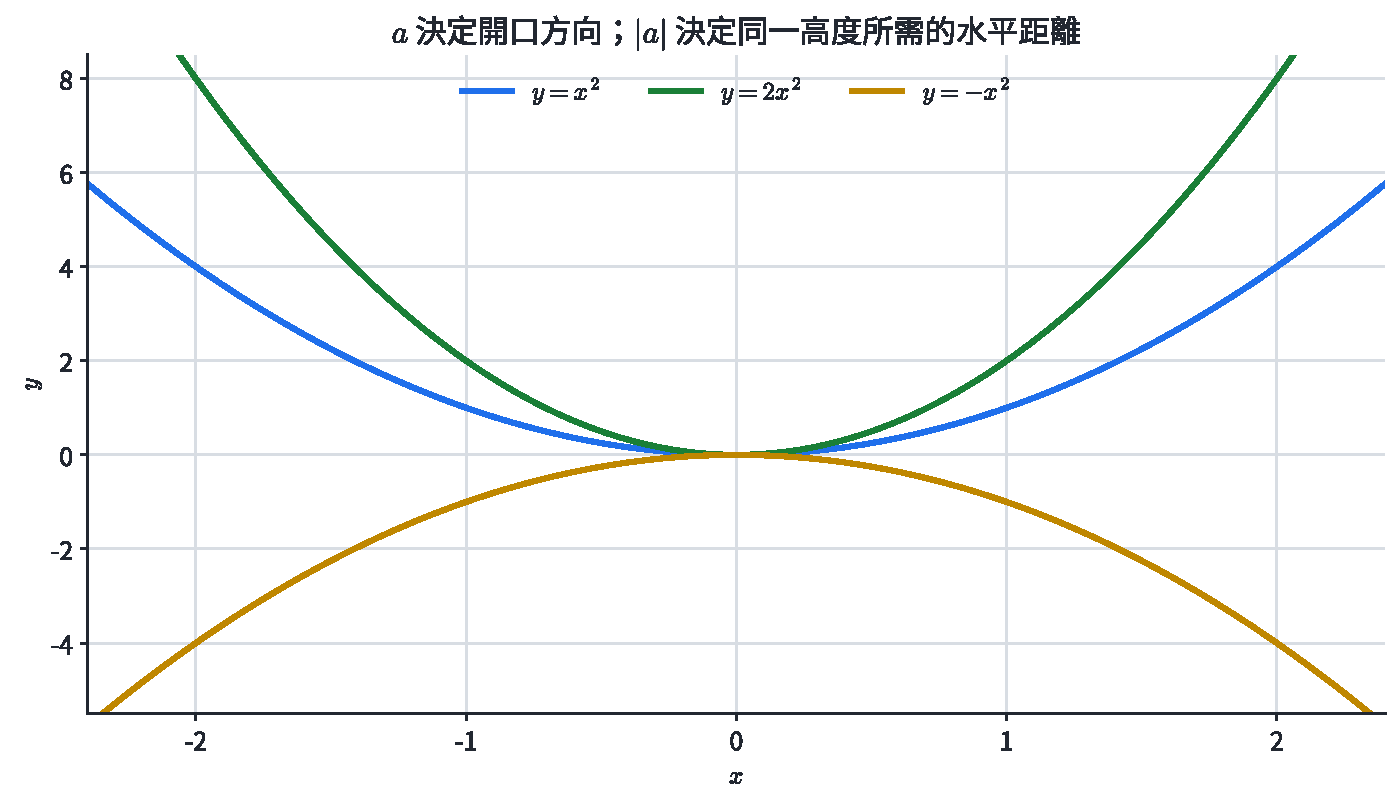
\includegraphics[width=0.88\linewidth,height=\textheight,keepaspectratio,alt={圖 4｜三條拋物線都以原點為頂點；開口方向與寬窄直接由 a 決定。}]{assets/數1-3-二次基本圖形.pdf}
\caption{圖 4｜三條拋物線都以原點為頂點；開口方向與寬窄直接由 \(a\) 決定。}
\end{figure}

將 \(y=ax^2\) 向右平移 \(h\)、向上平移 \(k\)，得到

\[
y=a(x-h)^2+k.
\]

理由是新圖上的輸入 \(x\) 對應到原圖的輸入 \(x-h\)；原輸出為 \(a(x-h)^2\)，再加上垂直位移 \(k\)。

\subsection{4.2 配方與頂點}\label{ux914dux65b9ux8207ux9802ux9ede}

一般式可配方為

\[
\begin{aligned}
ax^2+bx+c
&=a\left(x^2+\frac ba x\right)+c\\
&=a\left(x+\frac{b}{2a}\right)^2-\frac{b^2-4ac}{4a}.
\end{aligned}
\]

因此頂點與對稱軸為

\[
\boxed{\left(-\frac b{2a},-\frac{b^2-4ac}{4a}\right)},
\qquad
\boxed{x=-\frac b{2a}}.
\]

平方項的最小值是 \(0\)。當 \(a>0\)，頂點給全域最小值；當 \(a<0\)，頂點給全域最大值。

\subsection{例 9｜配方讀出圖形資訊}\label{ux4f8b-9ux914dux65b9ux8b80ux51faux5716ux5f62ux8cc7ux8a0a}

將 \(f(x)=2x^2-8x+5\) 配方，求頂點、對稱軸、最小值與 \(x\) 軸交點。

\[
f(x)=2(x^2-4x)+5=2(x-2)^2-3.
\]

頂點是 \((2,-3)\)，對稱軸是 \(x=2\)，最小值為 \(-3\)。令 \(f(x)=0\)：

\[
2(x-2)^2=3
\iff x=2\pm\frac{\sqrt6}{2}.
\]

\begin{figure}
\centering
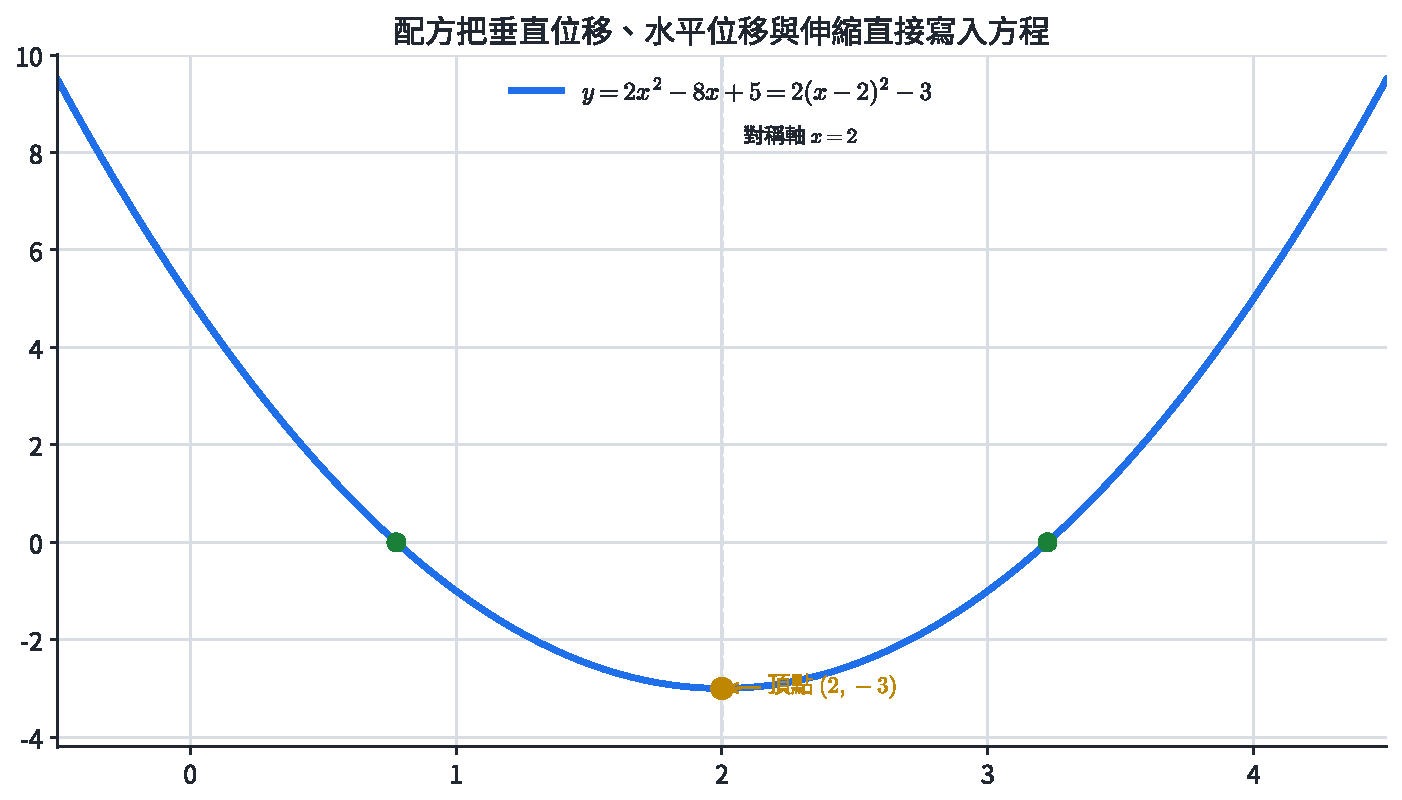
\includegraphics[width=0.88\linewidth,height=\textheight,keepaspectratio,alt={圖 5｜方程與圖形共用同一頂點、對稱軸與兩個精確根。}]{assets/數1-3-配方與頂點.pdf}
\caption{圖 5｜方程與圖形共用同一頂點、對稱軸與兩個精確根。}
\end{figure}

\subsection{4.3 判別式與交點}\label{ux5224ux5225ux5f0fux8207ux4ea4ux9ede}

方程 \(ax^2+bx+c=0\) 的判別式為 \(D=b^2-4ac\)。

\begin{itemize}
\tightlist
\item
  \(D>0\)：兩個相異實根，圖形穿越 \(x\) 軸兩次。
\item
  \(D=0\)：一個重根，圖形與 \(x\) 軸相切。
\item
  \(D<0\)：沒有實根，圖形與 \(x\) 軸沒有交點。
\end{itemize}

當 \(D<0\) 時，函數全程保持同號；其符號就是首項係數 \(a\) 的符號。

\begin{figure}
\centering
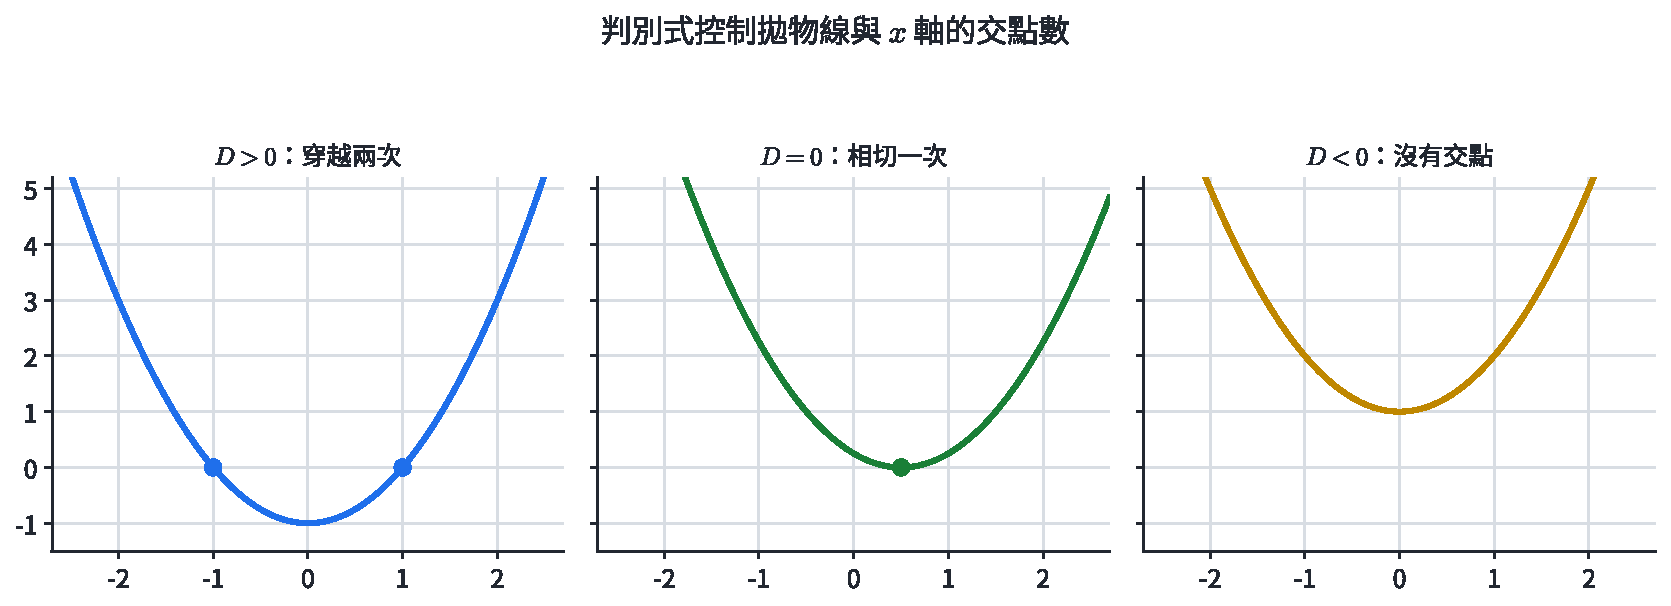
\includegraphics[width=0.94\linewidth,height=\textheight,keepaspectratio,alt={圖 6｜三個開口向上的二次函數，以交點數呈現判別式的三種情形。}]{assets/數1-3-判別式三情形.pdf}
\caption{圖 6｜三個開口向上的二次函數，以交點數呈現判別式的三種情形。}
\end{figure}

\subsection{例 10｜用判別式判斷全程符號}\label{ux4f8b-10ux7528ux5224ux5225ux5f0fux5224ux65b7ux5168ux7a0bux7b26ux865f}

判斷 \(g(x)=x^2+6x+11\) 的圖形與符號。

\[
g(x)=(x+3)^2+2,
\qquad D=36-44=-8<0.
\]

圖形開口向上且沒有 \(x\) 軸交點，所以對所有實數 \(x\)，皆有 \(\boxed{g(x)>0}\)。

\subsection{4.4 閉區間上的最大值與最小值}\label{ux9589ux5340ux9593ux4e0aux7684ux6700ux5927ux503cux8207ux6700ux5c0fux503c}

在閉區間 \([p,q]\) 上，二次函數的極值候選點是兩個端點，以及落在區間內的頂點。計算所有可取候選點的函數值後比較，即可得到最大值與最小值。

\subsection{例 11｜閉區間極值}\label{ux4f8b-11ux9589ux5340ux9593ux6975ux503c}

求 \(f(x)=x^2-4x+1\) 在 \([0,3]\) 上的最大值與最小值。

\[
f(x)=(x-2)^2-3.
\]

頂點 \(x=2\) 位於區間內。三個候選值為

\[
f(0)=1,\qquad f(2)=-3,\qquad f(3)=-2.
\]

所以最大值為 \(\boxed1\)，在 \(x=0\) 取得；最小值為 \(\boxed{-3}\)，在 \(x=2\) 取得。

\begin{figure}
\centering
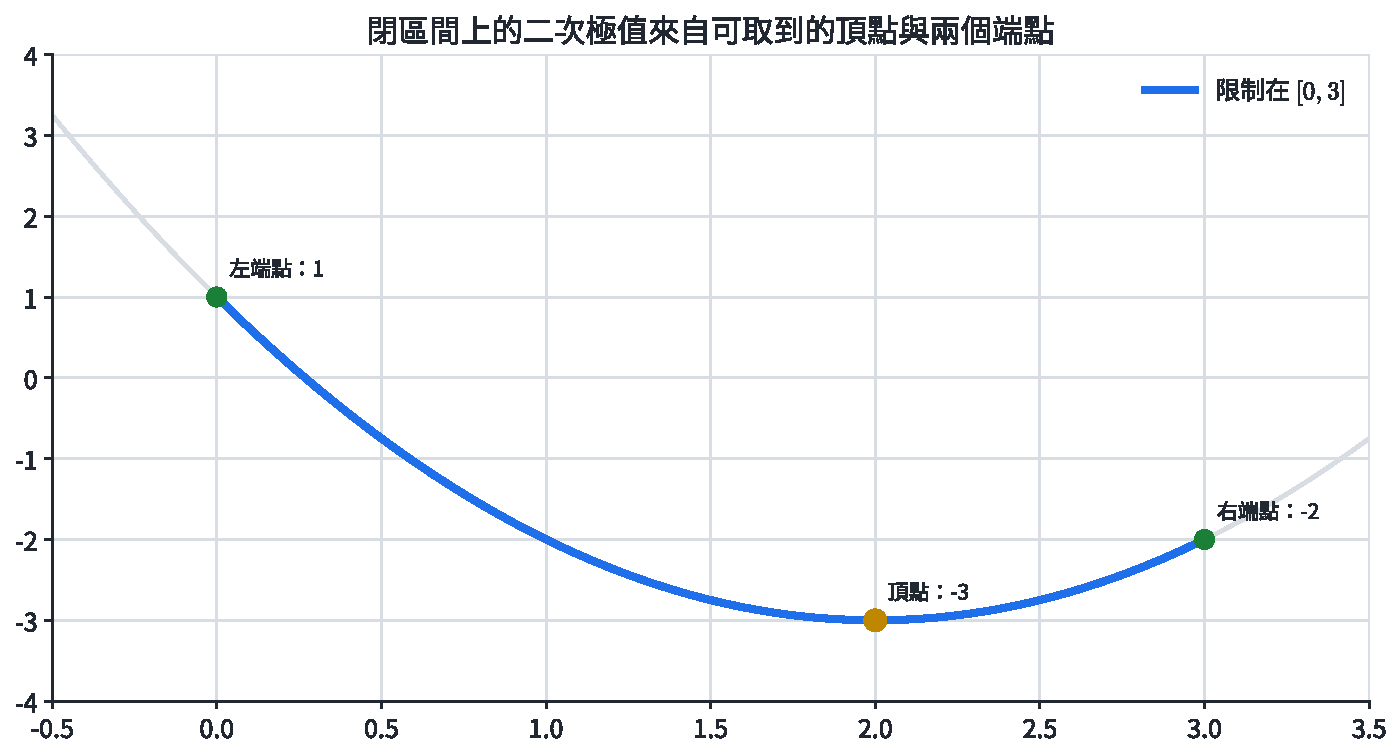
\includegraphics[width=0.88\linewidth,height=\textheight,keepaspectratio,alt={圖 7｜藍色曲線是可取的區間；三個標記點完整涵蓋極值候選。}]{assets/數1-3-閉區間極值.pdf}
\caption{圖 7｜藍色曲線是可取的區間；三個標記點完整涵蓋極值候選。}
\end{figure}

\subsection{例 12｜固定總長下的最大面積}\label{ux4f8b-12ux56faux5b9aux7e3dux9577ux4e0bux7684ux6700ux5927ux9762ux7a4d}

長方形兩邊長為 \(x\) 與 \(20-x\)，其中 \(0\le x\le20\)。求最大面積。

\[
A(x)=x(20-x)=-x^2+20x=-(x-10)^2+100.
\]

頂點 \(x=10\) 位於允許區間，故最大面積為 \(\boxed{100}\)，此時兩邊都長 \(10\)。

\subsubsection{練習 4A}\label{ux7df4ux7fd2-4a}

\begin{enumerate}
\def\labelenumi{\arabic{enumi}.}
\tightlist
\item
  對 \(y=-2(x+1)^2+5\)，求頂點、對稱軸、最大值與 \(x\) 軸交點。
\item
  配方並判斷 \(x^2+6x+11\) 的最小值與實根數。
\item
  求 \(-x^2+4x+5\) 在 \([-1,4]\) 上的最大值與最小值。
\item
  求 \(2x^2-12x+11\) 在 \([1,5]\) 上的最大值與最小值。
\item
  長方形周長為 \(40\)，設一邊長 \(x\)。建立面積函數並求最大面積。
\item
  求使 \(x^2+(m-2)x+m=0\) 有重根的 \(m\)。
\end{enumerate}

\section{5. 三次函數：標準形、平移與局部近似}\label{ux4e09ux6b21ux51fdux6578ux6a19ux6e96ux5f62ux5e73ux79fbux8207ux5c40ux90e8ux8fd1ux4f3c}

\subsection{5.1 三次標準形與大域特徵}\label{ux4e09ux6b21ux6a19ux6e96ux5f62ux8207ux5927ux57dfux7279ux5fb5}

三次標準形為 \(g(x)=ax^3+px\)，其中 \(a\ne0\)。因為 \(g(-x)=-g(x)\)，圖形關於原點點對稱。當 \(|x|\) 很大時，\(ax^3\) 的成長速度超過 \(px\)，因此兩端方向由 \(a\) 決定：

\begin{itemize}
\tightlist
\item
  \(a>0\)：左端向下、右端向上。
\item
  \(a<0\)：左端向上、右端向下。
\end{itemize}

在原點附近，\(g(x)=x(ax^2+p)\)。當 \(p\ne0\) 且 \(|x|\) 足夠小，括號的符號由 \(p\) 控制，所以 \(p\) 決定圖形穿過原點附近的方向。這是局部判讀；遠端仍由 \(a\) 控制。

\begin{figure}
\centering
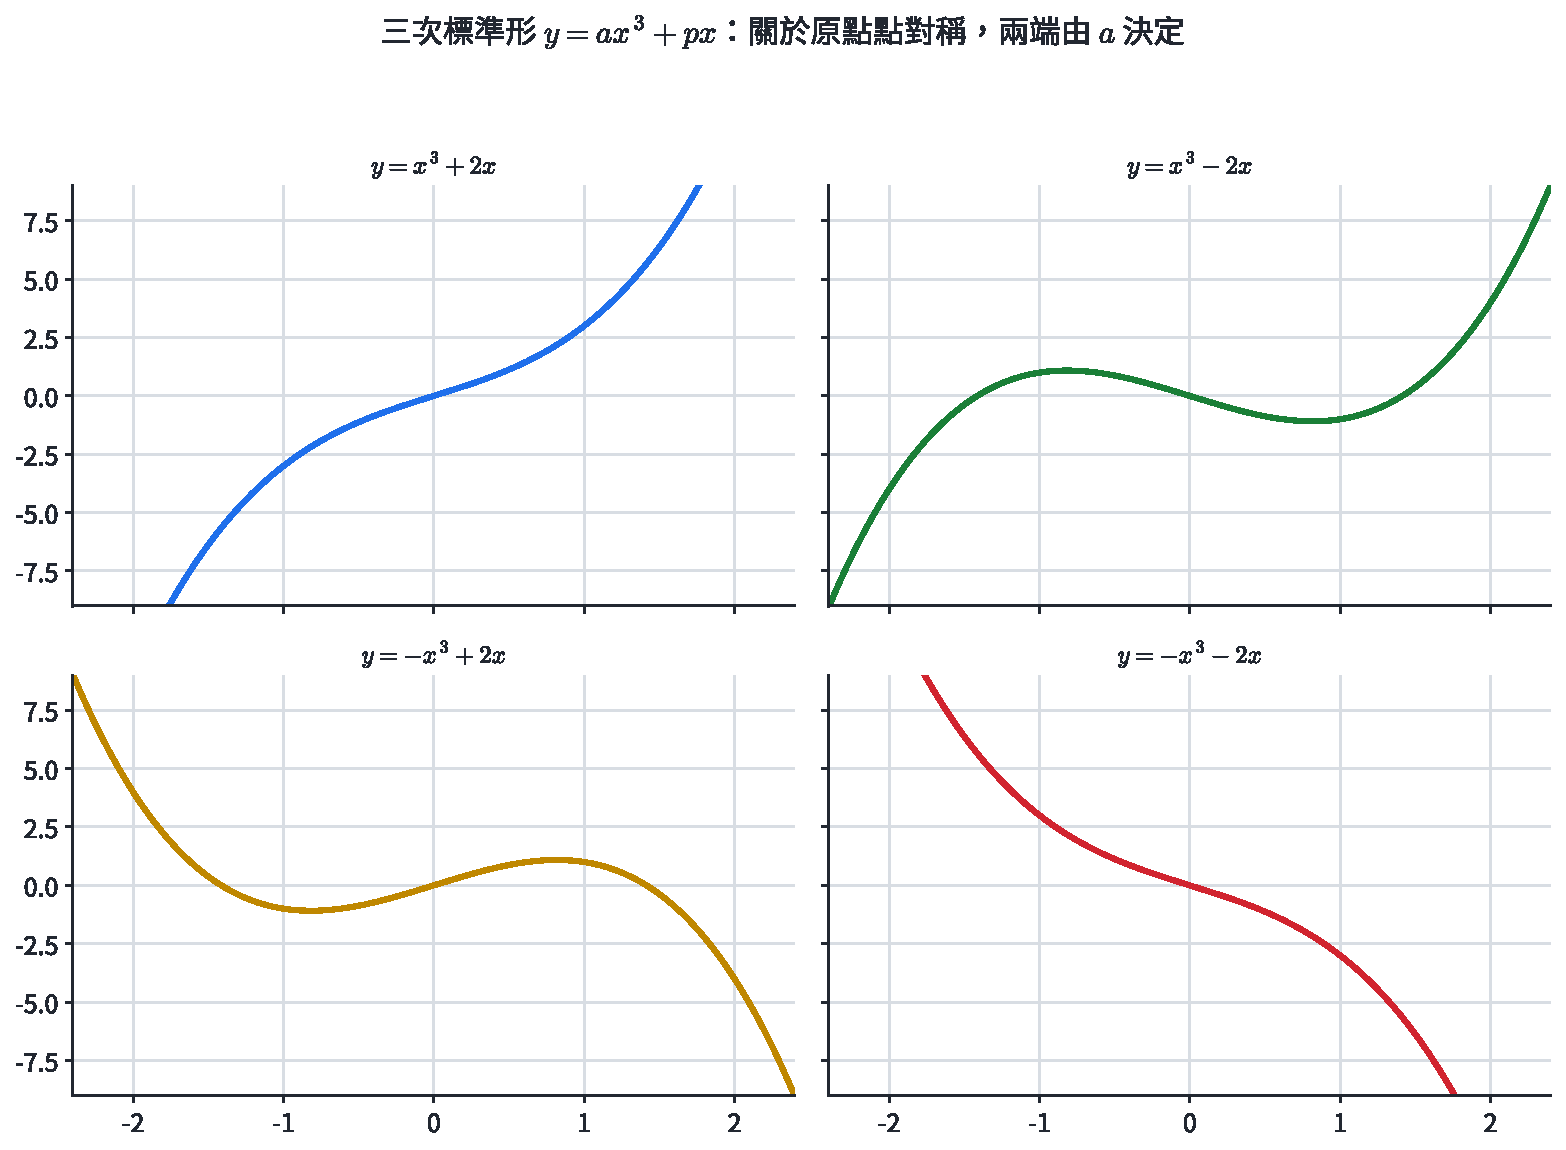
\includegraphics[width=0.88\linewidth,height=\textheight,keepaspectratio,alt={圖 8｜四組 a,p 皆關於原點點對稱；a 固定兩端，p 影響中心附近的走向。}]{assets/數1-3-三次標準形.pdf}
\caption{圖 8｜四組 \(a,p\) 皆關於原點點對稱；\(a\) 固定兩端，\(p\) 影響中心附近的走向。}
\end{figure}

\subsection{5.2 一般三次式化為平移標準形}\label{ux4e00ux822cux4e09ux6b21ux5f0fux5316ux70baux5e73ux79fbux6a19ux6e96ux5f62}

設 \(f(x)=ax^3+bx^2+cx+d\)。令 \(x=u+h\)。展開後，\(u^2\) 的係數為 \(3ah+b\)。選

\[
\boxed{h=-\frac b{3a}}
\]

便可消去二次項，得到

\[
f(x)=a(x-h)^3+p(x-h)+k.
\]

右側是標準形 \(au^3+pu\) 向右平移 \(h\)、向上平移 \(k\)，所以圖形的對稱中心為

\[
\boxed{(h,k)=(h,f(h))}.
\]

\subsection{例 13｜三次函數的平移與對稱中心}\label{ux4f8b-13ux4e09ux6b21ux51fdux6578ux7684ux5e73ux79fbux8207ux5c0dux7a31ux4e2dux5fc3}

將 \(f(x)=x^3-3x^2+2\) 化為平移標準形。

此處 \(a=1,b=-3\)，所以 \(h=1\)。令 \(u=x-1\)，即 \(x=u+1\)：

\[
f(x)=(u+1)^3-3(u+1)^2+2=u^3-3u.
\]

因此 \(\boxed{f(x)=(x-1)^3-3(x-1)}\)，對稱中心為 \((1,0)\)，大域走向為左下到右上。

\begin{figure}
\centering
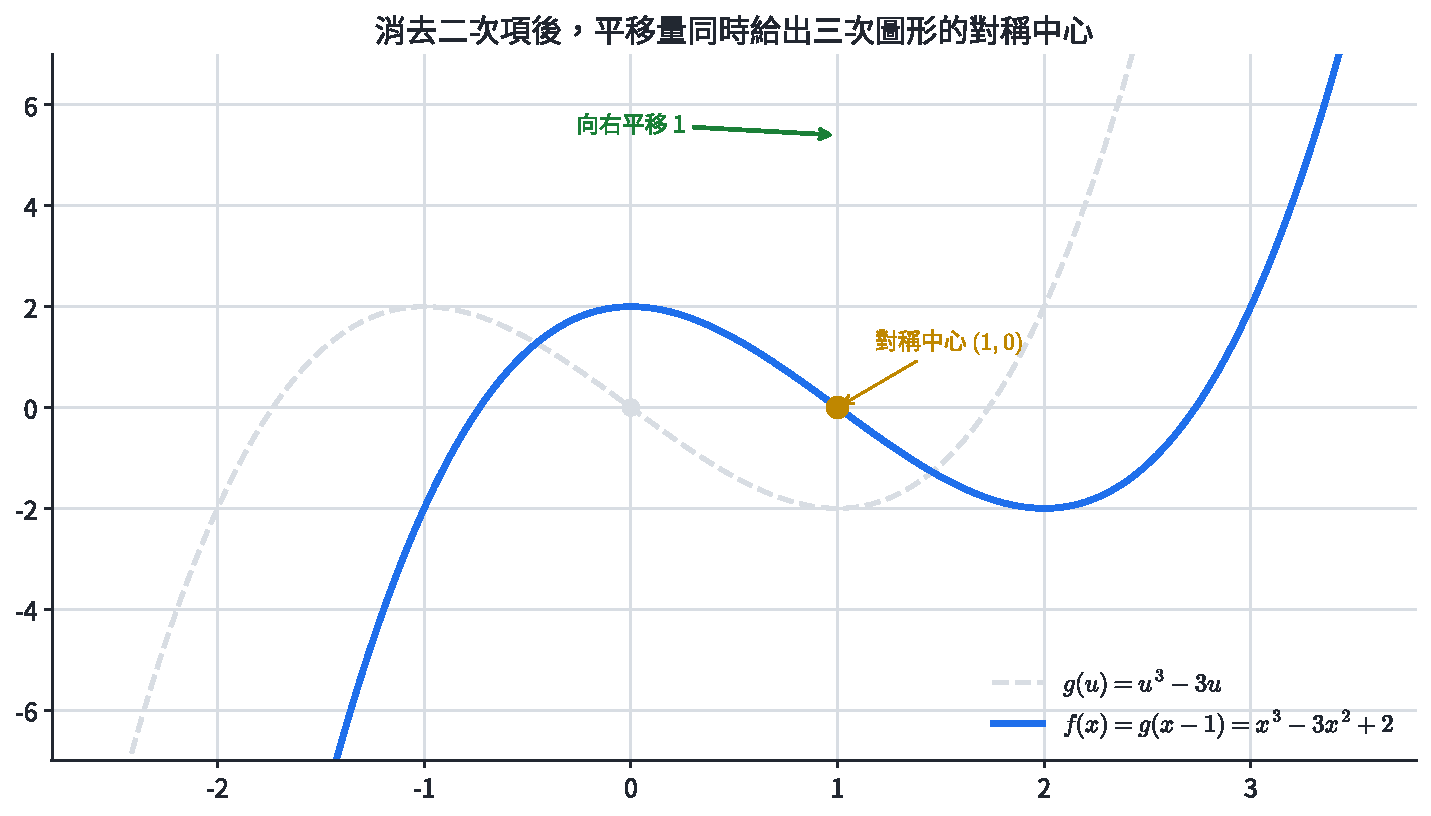
\includegraphics[width=0.88\linewidth,height=\textheight,keepaspectratio,alt={圖 9｜虛線標準形向右平移一單位後，原點移到對稱中心 (1,0)。}]{assets/數1-3-三次平移與對稱中心.pdf}
\caption{圖 9｜虛線標準形向右平移一單位後，原點移到對稱中心 \((1,0)\)。}
\end{figure}

\subsection{5.3 連續綜合除法與指定點的一次近似}\label{ux9023ux7e8cux7d9cux5408ux9664ux6cd5ux8207ux6307ux5b9aux9edeux7684ux4e00ux6b21ux8fd1ux4f3c}

連續用 \(x-h\) 做綜合除法，可以把 \(n\) 次多項式唯一寫成

\[
f(x)=c_0+c_1(x-h)+c_2(x-h)^2+\cdots+c_n(x-h)^n.
\]

第一次綜合除法的餘式是 \(c_0=f(h)\)；把第一次的商再除以 \(x-h\)，下一個餘式是 \(c_1\)；依序進行便得到所有係數。

當 \(x\) 很接近 \(h\)，位移 \(u=x-h\) 很小，\(u^2,u^3,\ldots\) 的量級迅速降低。保留前兩項可得局部一次近似

\[
\boxed{f(x)\approx c_0+c_1(x-h)}.
\]

近似的適用範圍由被省略的高次項控制；位移越小，誤差通常越小。

\subsection{例 14｜在指定點建立一次近似}\label{ux4f8b-14ux5728ux6307ux5b9aux9edeux5efaux7acbux4e00ux6b21ux8fd1ux4f3c}

對 \(f(x)=2x^3+6x^2+3x-3\) 在 \(h=-2\) 附近建立一次近似，並估算 \(f(-1.98)\)。

令 \(u=x+2\)。連續綜合除法或直接代換可得

\[
f(x)=2u^3-6u^2+3u-1.
\]

保留常數項與一次項：\(f(x)\approx3u-1=3(x+2)-1\)。當 \(x=-1.98\)，\(u=0.02\)，所以近似值為 \(\boxed{-0.94}\)。精確值為

\[
2(0.02)^3-6(0.02)^2+3(0.02)-1=-0.942384,
\]

誤差絕對值為 \(0.002384\)。

\begin{figure}
\centering
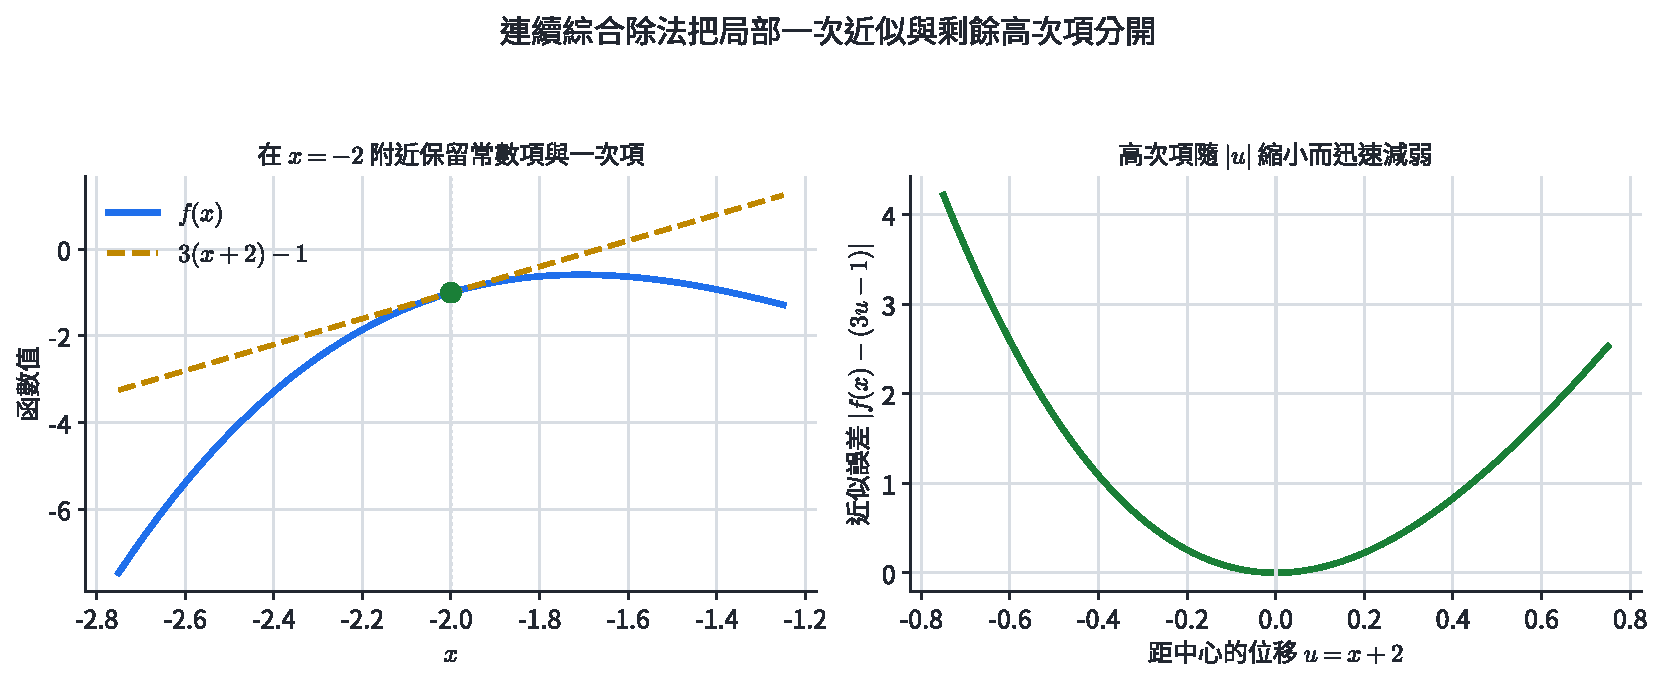
\includegraphics[width=0.94\linewidth,height=\textheight,keepaspectratio,alt={圖 10｜左圖比較函數與一次近似，右圖直接畫出誤差隨位移增加的變化。}]{assets/數1-3-局部一次近似.pdf}
\caption{圖 10｜左圖比較函數與一次近似，右圖直接畫出誤差隨位移增加的變化。}
\end{figure}

\subsubsection{練習 5A}\label{ux7df4ux7fd2-5a}

\begin{enumerate}
\def\labelenumi{\arabic{enumi}.}
\tightlist
\item
  將 \(2x^3+6x^2+3x-1\) 化為 \(2(x+1)^3+p(x+1)+k\)，並求對稱中心。
\item
  求 \(2x^3-12x^2+9x+5\) 的對稱中心與兩端走向。
\item
  將 \(x^3+3x^2-1\) 以 \(u=x+1\) 表示，寫出在 \(x=-1\) 附近的一次近似。
\item
  承上題，用一次近似估算 \(f(-0.95)\)，再計算精確值與誤差。
\item
  若 \(f(x)=a(x-h)^3+p(x-h)+k\)，證明 \(f(h+t)+f(h-t)=2k\)。
\end{enumerate}

\section{6. 多項式不等式與重根變號}\label{ux591aux9805ux5f0fux4e0dux7b49ux5f0fux8207ux91cdux6839ux8b8aux865f}

\subsection{6.1 一次與二次不等式}\label{ux4e00ux6b21ux8207ux4e8cux6b21ux4e0dux7b49ux5f0f}

一次不等式依等式的移項規則整理；兩邊同乘或同除負數時，不等號方向反轉。

二次不等式可轉成圖形相對於 \(x\) 軸的位置。若 \(a>0\) 且有兩相異根 \(\alpha<\beta\)，則

\[
ax^2+bx+c
\begin{cases}
>0,&x<\alpha\text{ 或 }x>\beta,\\
<0,&\alpha<x<\beta.
\end{cases}
\]

等號是否納入，由題目的 \(\ge,\le\) 決定。\(D=0\) 時函數只在重根處等於 \(0\)；\(D<0\) 時函數保持首項係數的符號。

\subsection{例 15｜一次與二次不等式}\label{ux4f8b-15ux4e00ux6b21ux8207ux4e8cux6b21ux4e0dux7b49ux5f0f}

解 \(-3x+6\le0\) 與 \(x^2-x-6<0\)。

第一題：\(-3x\le-6\)，同除以 \(-3\) 得 \(\boxed{x\ge2}\)。

第二題：\(x^2-x-6=(x+2)(x-3)\)。開口向上，兩根為 \(-2,3\)，負值位於兩根之間，所以解為 \(\boxed{-2<x<3}\)。

\subsection{例 16｜重根對二次不等式的影響}\label{ux4f8b-16ux91cdux6839ux5c0dux4e8cux6b21ux4e0dux7b49ux5f0fux7684ux5f71ux97ff}

解 \((x-2)^2\le0\)。

平方恆為非負數，等於 \(0\) 的條件是 \(x=2\)。因此解集為 \(\boxed{\{2\}}\)。

\subsection{6.2 可分解高次不等式}\label{ux53efux5206ux89e3ux9ad8ux6b21ux4e0dux7b49ux5f0f}

若

\[
P(x)=A\prod_i(x-r_i)^{m_i},
\]

各根 \(r_i\) 把數線分成若干區間。每個區間內沒有根，函數值會維持同號。跨過根時：

\begin{itemize}
\tightlist
\item
  \(m_i\) 為奇數，因式 \((x-r_i)^{m_i}\) 變號，整體符號翻轉。
\item
  \(m_i\) 為偶數，該因式兩側同號，整體符號保持。
\end{itemize}

先按大小排列根，從任一測試點取得一段符號，再依重數向左右推移即可。若題目含 \(\ge\) 或 \(\le\)，所有使乘積為零的根都要依條件納入。

\begin{figure}
\centering
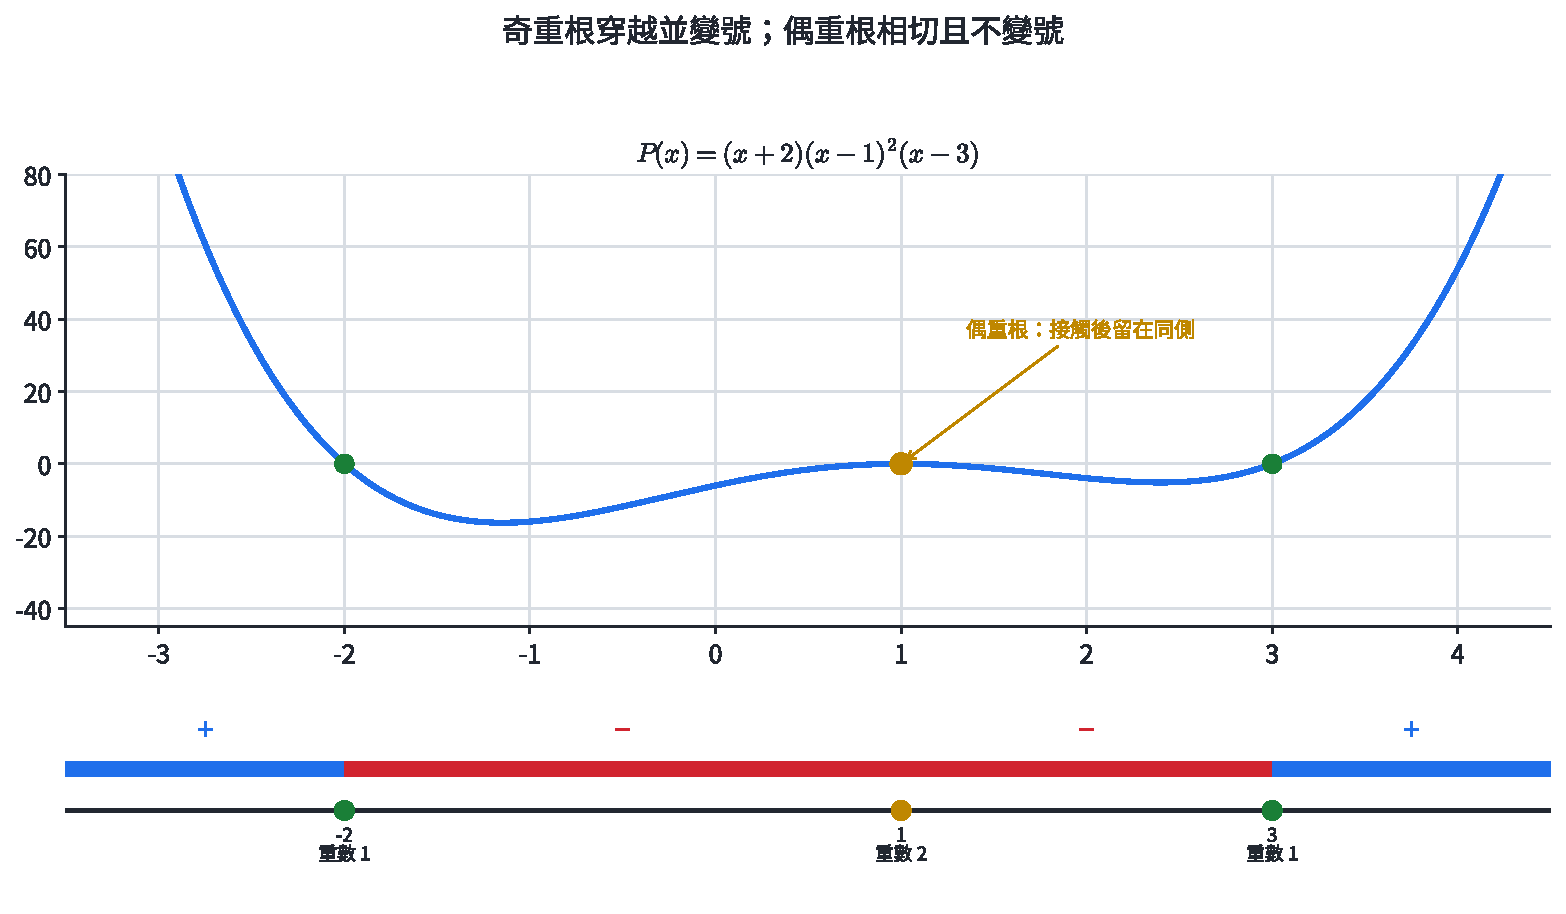
\includegraphics[width=0.92\linewidth,height=\textheight,keepaspectratio,alt={圖 11｜曲線在奇重根穿越 x 軸，在偶重根接觸後返回同側；下方符號線與曲線完全一致。}]{assets/數1-3-重根與變號.pdf}
\caption{圖 11｜曲線在奇重根穿越 \(x\) 軸，在偶重根接觸後返回同側；下方符號線與曲線完全一致。}
\end{figure}

\subsection{例 17｜含偶重根的高次不等式}\label{ux4f8b-17ux542bux5076ux91cdux6839ux7684ux9ad8ux6b21ux4e0dux7b49ux5f0f}

解 \((x+2)(x-1)^2(x-3)\ge0\)。

根依序為 \(-2,1,3\)，重數分別為 \(1,2,1\)。首項係數為正，最右側為正；跨過 \(3\) 變負，跨過偶重根 \(1\) 保持負，跨過 \(-2\) 再變正。非負區間加上所有根，得到

\[
\boxed{(-\infty,-2]\cup\{1\}\cup[3,\infty)}.
\]

\subsection{例 18｜先確認恆正因式}\label{ux4f8b-18ux5148ux78baux8a8dux6046ux6b63ux56e0ux5f0f}

解 \((x^2+1)(x-4)(x+1)<0\)。

因 \(x^2+1>0\) 對所有實數成立，乘積符號由 \((x-4)(x+1)\) 決定。開口向上的二次式在兩根 \(-1,4\) 之間為負，所以 \(\boxed{-1<x<4}\)。

\subsubsection{練習 6A}\label{ux7df4ux7fd2-6a}

\begin{enumerate}
\def\labelenumi{\arabic{enumi}.}
\tightlist
\item
  解 \(-4x+12>0\)。
\item
  解 \(x^2-5x+6\le0\)。
\item
  解 \(2x^2+4x+5>0\)。
\item
  解 \(-(x-1)(x+2)>0\)。
\item
  解 \((x+3)x(2x-1)\le0\)。
\item
  解 \((x-2)^2(x+1)<0\)。
\end{enumerate}

\section{7. 分節練習完整解析}\label{ux5206ux7bc0ux7df4ux7fd2ux5b8cux6574ux89e3ux6790}

\subsection{練習 1A}\label{ux7df4ux7fd2-1a-1}

\begin{enumerate}
\def\labelenumi{\arabic{enumi}.}
\tightlist
\item
  \(3x^4-\sqrt2x+1\) 為四次多項式，首項係數 \(3\)、常數項 \(1\)。\(x^{-1}+2\) 含負整數指數，\(\sqrt{x}+1\) 含分數指數，兩式都不符合多項式定義。
\item
  比較三次與二次項係數：\(a-1=0\)、\(b+2=0\)，故 \(\boxed{a=1,b=-2}\)。
\item
  依分配律展開得 \(\boxed{2x^3-5x^2+5x-6}\)。
\item
  三次項相消，\(f+g=\boxed{x^2-2x+5}\)，次數為 \(2\)。
\item
  \(C(3)=2(27)-5(3)+12=\boxed{51}\)。
\end{enumerate}

\subsection{練習 2A}\label{ux7df4ux7fd2-2a-1}

\begin{enumerate}
\def\labelenumi{\arabic{enumi}.}
\tightlist
\item
  \(x^4-1=(x^2+1)(x^2-1)\)，故商為 \(\boxed{x^2-1}\)，餘式為 \(0\)。
\item
  對 \(a=-1\) 做綜合除法，係數 \(3,0,-2,0,7\) 得底列 \(3,-3,1,-1,8\)。商為 \(\boxed{3x^3-3x^2+x-1}\)，餘式為 \(\boxed8\)。
\item
  除式 \(2x-1\) 的零點為 \(1/2\)。餘式為
  \[2\left(\frac12\right)^5-3\left(\frac12\right)+4=\boxed{\frac{41}{16}}.\]
\item
  因式定理給 \(8+4a-10+6=0\)，所以 \(\boxed{a=-1}\)。
\item
  設餘式 \(mx+n\)。由 \(m+n=2\)、\(-2m+n=-4\) 得 \(m=2,n=0\)，故餘式為 \(\boxed{2x}\)。
\item
  整除 \(x^2-1=(x-1)(x+1)\) 給 \(f(1)=f(-1)=0\)：
  \[2+2a+b=0,\qquad2-2a+b=0.\]
  相減得 \(a=0\)，再得 \(b=-2\)。故 \(\boxed{a=0,b=-2}\)。
\end{enumerate}

\subsection{練習 3A}\label{ux7df4ux7fd2-3a-1}

\begin{enumerate}
\def\labelenumi{\arabic{enumi}.}
\tightlist
\item
  依序為 \(\boxed{(-3,-4),(3,4),(3,-4),(4,-3)}\)。
\item
  中點為 \(\left((-2+6)/2,(5-1)/2\right)=\boxed{(2,2)}\)。
\item
  \(y^2=x\) 在 \(x=4\) 對應 \(y=\pm2\)；\(x^2+y^2=1\) 在多數 \(x\in(-1,1)\) 對應兩個 \(y\)，所以兩者都未把 \(y\) 定為 \(x\) 的函數。\(y=|x|\) 對每個實數 \(x\) 有唯一輸出，故為函數。
\item
  斜率 \(m=(-3-5)/(3+1)=-2\)。代入 \((-1,5)\) 得 \(b=3\)，所以 \(f(x)=\boxed{-2x+3}\)，\(f(2)=\boxed{-1}\)。
\item
  \(C(x)=\boxed{8.5x+45}\)，\(C(12)=102+45=\boxed{147}\) 元。
\end{enumerate}

\subsection{練習 4A}\label{ux7df4ux7fd2-4a-1}

\begin{enumerate}
\def\labelenumi{\arabic{enumi}.}
\tightlist
\item
  頂點 \((-1,5)\)，對稱軸 \(x=-1\)，最大值 \(5\)。令 \(-2(x+1)^2+5=0\)，得交點 \(x=\boxed{-1\pm\sqrt{5/2}}\)。
\item
  \(x^2+6x+11=(x+3)^2+2\)，最小值為 \(\boxed2\)；判別式 \(-8<0\)，故實根數為 \(0\)。
\item
  \(-x^2+4x+5=-(x-2)^2+9\)。候選值 \(f(-1)=0,f(2)=9,f(4)=5\)，故最大值 \(\boxed9\)，最小值 \(\boxed0\)。
\item
  \(2x^2-12x+11=2(x-3)^2-7\)。候選值 \(f(1)=1,f(3)=-7,f(5)=1\)，故最大值 \(\boxed1\)，最小值 \(\boxed{-7}\)。
\item
  另一邊為 \(20-x\)，\(A(x)=x(20-x)=-(x-10)^2+100\)，故最大面積為 \(\boxed{100}\)。
\item
  重根條件 \(D=0\)：
  \[(m-2)^2-4m=m^2-8m+4=0,\]
  所以 \(\boxed{m=4\pm2\sqrt3}\)。
\end{enumerate}

\subsection{練習 5A}\label{ux7df4ux7fd2-5a-1}

\begin{enumerate}
\def\labelenumi{\arabic{enumi}.}
\tightlist
\item
  令 \(u=x+1\)，展開得 \(2u^3-3u\)，故 \(p=-3,k=0\)，對稱中心為 \(\boxed{(-1,0)}\)。
\item
  \(h=-(-12)/(3\cdot2)=2\)，\(k=f(2)=16-48+18+5=-9\)，中心為 \(\boxed{(2,-9)}\)。首項係數為正，兩端為左下、右上。
\item
  令 \(u=x+1\)，則 \(f(x)=u^3-3u+1\)，一次近似為 \(\boxed{1-3u=1-3(x+1)}\)。
\item
  \(u=0.05\)，近似值 \(1-3(0.05)=0.85\)；精確值 \(0.05^3-3(0.05)+1=0.850125\)，誤差為 \(\boxed{0.000125}\)。
\item
  直接代入：
  \[f(h+t)=at^3+pt+k,\qquad f(h-t)=-at^3-pt+k.\]
  相加得 \(\boxed{2k}\)，這正是以 \((h,k)\) 為中點的數值對稱。
\end{enumerate}

\subsection{練習 6A}\label{ux7df4ux7fd2-6a-1}

\begin{enumerate}
\def\labelenumi{\arabic{enumi}.}
\tightlist
\item
  \(-4x>-12\)，同除以 \(-4\) 得 \(\boxed{x<3}\)。
\item
  \((x-2)(x-3)\le0\)，解為 \(\boxed{[2,3]}\)。
\item
  判別式 \(16-40=-24<0\) 且開口向上，故解為 \(\boxed{\mathbb R}\)。
\item
  等價於 \((x-1)(x+2)<0\)，解為 \(\boxed{(-2,1)}\)。
\item
  根為 \(-3,0,1/2\)，皆為奇重根。符號由最右側向左依序翻轉，解為 \(\boxed{(-\infty,-3]\cup[0,1/2]}\)。
\item
  偶次因式 \((x-2)^2\) 在 \(x=2\) 兩側保持正號，整體負號出現在 \(x+1<0\)，故解為 \(\boxed{(-\infty,-1)}\)。
\end{enumerate}

\section{8. 章末代表題}\label{ux7ae0ux672bux4ee3ux8868ux984c}

\subsection{基礎與核心（第 1--12 題）}\label{ux57faux790eux8207ux6838ux5fc3ux7b2c-112-ux984c}

\begin{enumerate}
\def\labelenumi{\arabic{enumi}.}
\tightlist
\item
  若 \((m-2)x^4+(n+1)x^2+3\) 恆等於常數 \(3\)，求 \(m,n\)。
\item
  設 \(f(x)=2x^2-x+1\)、\(g(x)=x-3\)，求 \(f(x)g(x)\)。
\item
  用綜合除法求 \((2x^3+x^2-5)\div(x+2)\) 的商與餘式。
\item
  求 \(x^5-3x+2\) 除以 \(2x+1\) 的餘式。
\item
  點 \(P(2,-5)\) 關於 \(y=x\) 與原點的像點各為何？
\item
  一次函數通過 \((1,4)\)、\((5,16)\)。求函數式與 \(f(8)\)。
\item
  將 \(-2x^2+8x-3\) 配方，求頂點、最大值與兩個零點。
\item
  求第 7 題函數在 \([0,3]\) 上的最大值與最小值。
\item
  將 \(2x^3-6x^2-3x+7\) 化為平移標準形，求對稱中心與兩端走向。
\item
  將 \(f(x)=x^3+2x^2-x+4\) 以 \(u=x-1\) 展開，寫出 \(x=1\) 附近的一次近似，並估算 \(f(1.02)\)。
\item
  解 \(2x^2-x-3\ge0\)。
\item
  解 \((x+1)^2(x-2)(x-4)<0\)。
\end{enumerate}

\subsection{跨節整合（第 13--16 題）}\label{ux8de8ux7bc0ux6574ux5408ux7b2c-1316-ux984c}

\begin{enumerate}
\def\labelenumi{\arabic{enumi}.}
\setcounter{enumi}{12}
\tightlist
\item
  一首項係數為 \(1\) 的三次多項式滿足 \(f(1)=f(-2)=0\)、\(f(0)=12\)，第三個根為實數。求 \(f(x)\)，並解 \(f(x)\le0\)。
\item
  某商品售出 \(x\) 件時，每件價格為 \(80-2x\) 元，且 \(0\le x\le40\)。建立收益函數，求最大收益與對應售價。
\item
  對 \(f(x)=2x^3+6x^2+3x-3\)，用連續綜合除法在 \(x=-2\) 附近建立一次近似。估算 \(f(-1.98)\)，並以高次項算出誤差。
\item
  三次式 \(f(x)=x^3+ax^2+bx+6\) 可被 \((x-1)(x+2)\) 整除。求 \(a,b\)，再解 \(f(x)\ge0\)。
\end{enumerate}

\section{9. 章末代表題完整詳解}\label{ux7ae0ux672bux4ee3ux8868ux984cux5b8cux6574ux8a73ux89e3}

\subsection{第 1 題}\label{ux7b2c-1-ux984c}

恆等於常數表示四次項與二次項係數皆為 \(0\)：

\[
m-2=0,\qquad n+1=0.
\]

故 \(\boxed{m=2,n=-1}\)。

\subsection{第 2 題}\label{ux7b2c-2-ux984c}

\[
\begin{aligned}
(2x^2-x+1)(x-3)
&=2x^3-6x^2-x^2+3x+x-3\\
&=\boxed{2x^3-7x^2+4x-3}.
\end{aligned}
\]

\subsection{第 3 題}\label{ux7b2c-3-ux984c}

除式 \(x+2=x-(-2)\)。係數 \(2,1,0,-5\) 以 \(-2\) 綜合除法，底列為 \(2,-3,6,-17\)。因此

\[
\boxed{q(x)=2x^2-3x+6,\qquad r=-17}.
\]

\subsection{第 4 題}\label{ux7b2c-4-ux984c}

\(2x+1\) 的零點為 \(-1/2\)。依餘式定理：

\[
\left(-\frac12\right)^5-3\left(-\frac12\right)+2
=-\frac1{32}+\frac32+2
=\boxed{\frac{111}{32}}.
\]

\subsection{第 5 題}\label{ux7b2c-5-ux984c}

關於 \(y=x\) 時交換坐標，得到 \(\boxed{(-5,2)}\)；關於原點時兩坐標同時變號，得到 \(\boxed{(-2,5)}\)。

\subsection{第 6 題}\label{ux7b2c-6-ux984c}

\[
m=\frac{16-4}{5-1}=3.
\]

代入 \((1,4)\) 得 \(4=3+b\)，故 \(b=1\)。函數為 \(\boxed{f(x)=3x+1}\)，並且 \(f(8)=24+1=\boxed{25}\)。

\subsection{第 7 題}\label{ux7b2c-7-ux984c}

\[
-2x^2+8x-3=-2(x-2)^2+5.
\]

頂點為 \((2,5)\)，最大值為 \(5\)。令函數值為 \(0\)：

\[
-2(x-2)^2+5=0
\iff (x-2)^2=\frac52,
\]

所以零點為 \(\boxed{x=2\pm\sqrt{10}/2}\)。

\subsection{第 8 題}\label{ux7b2c-8-ux984c}

頂點 \(x=2\) 位於 \([0,3]\)。候選值為

\[
f(0)=-3,\qquad f(2)=5,\qquad f(3)=3.
\]

故最大值為 \(\boxed5\)，最小值為 \(\boxed{-3}\)。

\subsection{第 9 題}\label{ux7b2c-9-ux984c}

\(a=2,b=-6\)，所以

\[
h=-\frac{-6}{3\cdot2}=1.
\]

令 \(u=x-1\)，即 \(x=u+1\)，展開得

\[
2x^3-6x^2-3x+7=2u^3-9u.
\]

因此 \(\boxed{f(x)=2(x-1)^3-9(x-1)}\)，對稱中心為 \(\boxed{(1,0)}\)。首項係數為正，兩端為左下、右上。

\subsection{第 10 題}\label{ux7b2c-10-ux984c}

令 \(u=x-1\)，則 \(x=u+1\)：

\[
\begin{aligned}
f(x)&=(u+1)^3+2(u+1)^2-(u+1)+4\\
&=u^3+5u^2+6u+6.
\end{aligned}
\]

一次近似為 \(\boxed{f(x)\approx6+6u=6+6(x-1)}\)。當 \(x=1.02\)，\(u=0.02\)：

\[
f(1.02)\approx6+6(0.02)=\boxed{6.12}.
\]

精確值為 \(6.122008\)，兩者相差 \(0.002008\)。

\subsection{第 11 題}\label{ux7b2c-11-ux984c}

\[
2x^2-x-3=(2x-3)(x+1).
\]

開口向上，兩根為 \(-1,3/2\)，非負值位於兩根外側並含根：

\[
\boxed{(-\infty,-1]\cup[3/2,\infty)}.
\]

\subsection{第 12 題}\label{ux7b2c-12-ux984c}

根為 \(-1,2,4\)，其中 \(-1\) 是偶重根。\((x+1)^2\) 在 \(x=-1\) 兩側同號，乘積的負號由 \((x-2)(x-4)\) 決定，位於兩根之間。因此 \(\boxed{(2,4)}\)。

\subsection{第 13 題｜因式資訊與符號分析}\label{ux7b2c-13-ux984cux56e0ux5f0fux8cc7ux8a0aux8207ux7b26ux865fux5206ux6790}

由因式定理，設

\[
f(x)=(x-1)(x+2)(x-r).
\]

代入 \(x=0\)：\(2r=12\)，故 \(r=6\)，

\[
\boxed{f(x)=(x-1)(x+2)(x-6)}.
\]

三個根依序為 \(-2,1,6\)，皆為奇重根；首項係數為正，所以符號由右向左依序為正、負、正、負。非正區間含各根：

\[
\boxed{(-\infty,-2]\cup[1,6]}.
\]

\subsection{第 14 題｜收益模型與閉區間極值}\label{ux7b2c-14-ux984cux6536ux76caux6a21ux578bux8207ux9589ux5340ux9593ux6975ux503c}

收益等於件數乘單價：

\[
R(x)=x(80-2x)=-2x^2+80x=-2(x-20)^2+800.
\]

頂點 \(x=20\) 位於 \([0,40]\)，故最大收益為 \(\boxed{800}\) 元。此時每件售價為

\[
80-2(20)=\boxed{40}\text{ 元}.
\]

\subsection{第 15 題｜局部展開與誤差}\label{ux7b2c-15-ux984cux5c40ux90e8ux5c55ux958bux8207ux8aa4ux5dee}

以 \(u=x+2\) 做連續綜合除法，得到

\[
f(x)=2u^3-6u^2+3u-1.
\]

一次近似為 \(3u-1\)。當 \(x=-1.98\)，\(u=0.02\)：

\[
f(-1.98)\approx3(0.02)-1=\boxed{-0.94}.
\]

被省略的高次項為

\[
2u^3-6u^2=2(0.02)^3-6(0.02)^2=-0.002384.
\]

因此精確值為 \(-0.942384\)，近似誤差的絕對值為 \(\boxed{0.002384}\)。

\subsection{第 16 題｜整除條件與三次不等式}\label{ux7b2c-16-ux984cux6574ux9664ux689dux4ef6ux8207ux4e09ux6b21ux4e0dux7b49ux5f0f}

整除 \((x-1)(x+2)\) 等價於 \(f(1)=f(-2)=0\)：

\[
1+a+b+6=0,
\]

\[
-8+4a-2b+6=0.
\]

整理得 \(a+b=-7\)、\(2a-b=1\)，解得 \(\boxed{a=-2,b=-5}\)。所以

\[
f(x)=x^3-2x^2-5x+6=(x-1)(x+2)(x-3).
\]

三個根 \(-2,1,3\) 都是奇重根，首項係數為正。非負區間為

\[
\boxed{[-2,1]\cup[3,\infty)}.
\]

\section{10. 核心整理}\label{ux6838ux5fc3ux6574ux7406}

\begin{enumerate}
\def\labelenumi{\arabic{enumi}.}
\tightlist
\item
  多項式的指數是非負整數；相等多項式逐次方比較係數。
\item
  除法原理是 \(f=gq+r\)，餘式次數低於除式；除以 \(x-a\) 時，餘式為 \(f(a)\)。
\item
  \(f(a)=0\) 等價於 \(x-a\) 是因式。二次除式的線性餘式可由兩個函數值決定。
\item
  二次函數配方後可直接讀出頂點、對稱軸與全域極值；閉區間另比較兩端點與區間內頂點。
\item
  判別式決定二次函數與 \(x\) 軸的交點數，也決定二次不等式的解集型態。
\item
  一般三次式以 \(h=-b/(3a)\) 平移後消去二次項，對稱中心為 \((h,f(h))\)；遠端由最高次項決定。
\item
  連續綜合除法可建立以 \(x-h\) 為基底的展開；靠近 \(h\) 時保留常數項與一次項得到局部近似。
\item
  多項式不等式先找根並依重數判斷變號：奇重根變號，偶重根保持符號。
\end{enumerate}


\end{document}
